
%----------------------------------------------------------------------------------------
%	PACKAGES AND OTHER DOCUMENT CONFIGURATIONS
%----------------------------------------------------------------------------------------

\documentclass[final]{beamer}

\usepackage[scale=1.24]{beamerposter} % Use the beamerposter package for laying out the poster

%\usetheme{confposter} % Use the confposter theme supplied with this template
\usetheme[faculty=chemo]{fibeamer} % Uncomment to use Masaryk University's fibeamer theme instead.

%\setbeamercolor{block title}{fg=ngreen,bg=white} % Colors of the block titles
%\setbeamercolor{block body}{fg=black,bg=white} % Colors of the body of blocks
%\setbeamercolor{block alerted title}{fg=white,bg=dblue!70} % Colors of the highlighted block titles
%\setbeamercolor{block alerted body}{fg=black,bg=dblue!10} % Colors of the body of highlighted blocks
% Many more colors are available for use in beamerthemeconfposter.sty

%-----------------------------------------------------------
% Define the column widths and overall poster size
% To set effective sepwid, onecolwid and twocolwid values, first choose how many columns you want and how much separation you want between columns
% In this template, the separation width chosen is 0.024 of the paper width and a 4-column layout
% onecolwid should therefore be (1-(# of columns+1)*sepwid)/# of columns e.g. (1-(4+1)*0.024)/4 = 0.22
% Set twocolwid to be (2*onecolwid)+sepwid = 0.464
% Set threecolwid to be (3*onecolwid)+2*sepwid = 0.708

\newlength{\sepwid}
\newlength{\onecolwid}
\newlength{\twocolwid}
\newlength{\threecolwid}
\setlength{\paperwidth}{46.8in} % A0 width: 46.8in
\setlength{\paperheight}{33.1in} % A0 height: 33.1in
\setlength{\sepwid}{0.024\paperwidth} % Separation width (white space) between columns
\setlength{\onecolwid}{0.21\paperwidth} % Width of one column
\setlength{\twocolwid}{0.451\paperwidth} % Width of two columns
\setlength{\threecolwid}{0.678\paperwidth} % Width of three columns
%\setlength{\topmargin}{-0.5in} % Reduce the top margin size
%-----------------------------------------------------------

\usepackage{graphicx}  % Required for including images

\usepackage{booktabs} % Top and bottom rules for tables

%----------------------------------------------------------------------------------------
%	TITLE SECTION 
%----------------------------------------------------------------------------------------

\title{Scientific Calculator} % Poster title

\author{Anand Kacha (40047673)} % Author(s)

\institute{Department of Computer Science and Engineering, Concordia University} % Institution(s)

%----------------------------------------------------------------------------------------

\begin{document}
\addtobeamertemplate{block end}{}{\vspace*{2ex}} % White space under blocks
\addtobeamertemplate{block example end}{}{\vspace*{2ex}} % White space under example blocks
\addtobeamertemplate{block alerted end}{}{\vspace*{2ex}} % White space under highlighted (alert) blocks

\setlength{\belowcaptionskip}{2ex} % White space under figures
\setlength\belowdisplayshortskip{2ex} % White space under equations
%\begin{darkframes} % Uncomment for dark theme, don't forget to \end{darkframes}
\begin{frame} % The whole poster is enclosed in one beamer frame

%==========================Begin Head===============================
  \begin{columns}
   \begin{column}{\linewidth}
    \vskip1cm
    \centering
    \usebeamercolor{title in headline}{\color{fg}\Huge{\textbf{\inserttitle}}\\[0.5ex]}
    \usebeamercolor{author in headline}{\color{fg}\Large{\insertauthor}\\[1ex]}
    \usebeamercolor{institute in headline}{\color{fg}\large{\insertinstitute}\\[1ex]}
    \vskip1cm
   \end{column}
   \vspace{1cm}
  \end{columns}
 \vspace{1cm}

%==========================End Head===============================

\begin{columns}[t] % The whole poster consists of three major columns, the second of which is split into two columns twice - the [t] option aligns each column's content to the top

\begin{column}{\sepwid}\end{column} % Empty spacer column

\begin{column}{\onecolwid} % The first column

%----------------------------------------------------------------------------------------
%	OBJECTIVES
%----------------------------------------------------------------------------------------

\begin{exampleblock}{Objectives}

The purpose of the project is to carry out a number of activities, resulting in a set of interrelated artifacts of a calculator:

\begin{itemize}
\item Research about the problem domain
\item Interview the potential users
\item Brainstorm and mind map with the team to create a persona
\item Construct UMLs for the problem domain
\item Design the user stories
\item Construct the backward Traceability Matrix
\item Begin the development of the calculator
\end{itemize}

\end{exampleblock}

%----------------------------------------------------------------------------------------
%	INTRODUCTION
%----------------------------------------------------------------------------------------

\begin{exampleblock}{}

\centering
\vspace{1em}
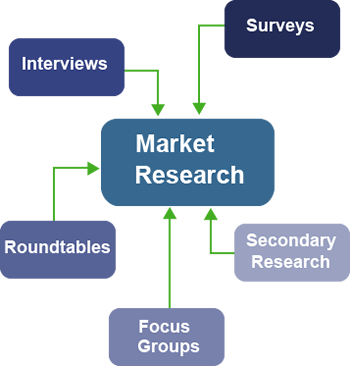
\includegraphics[width=0.7\linewidth]{img/market-research.png}
\vspace{1em}
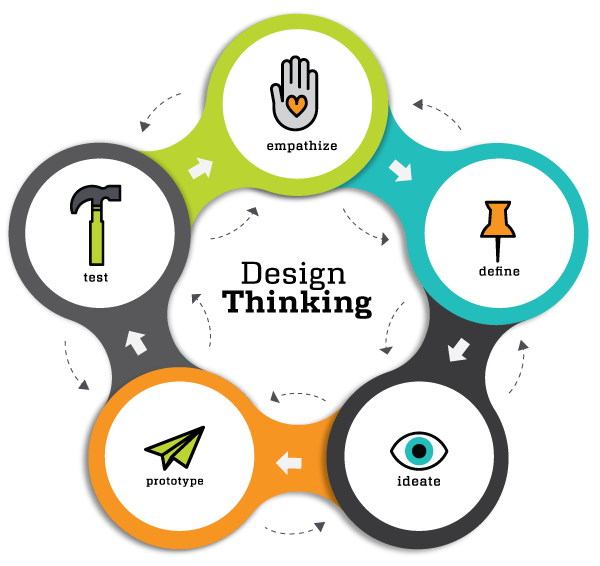
\includegraphics[scale=1]{img/design_thinking_visual.png}

\end{exampleblock}

%-----------------------------------------------

%----------------------------------------------------------------------------------------

\end{column} % End of the first column

\begin{column}{\sepwid}\end{column} % Empty spacer column

\begin{column}{\twocolwid} % Begin a column which is two columns wide (column 2)



%----------------------------------------------------------------------------------------
%	IMPORTANT RESULT
%----------------------------------------------------------------------------------------

\vspace{1em}
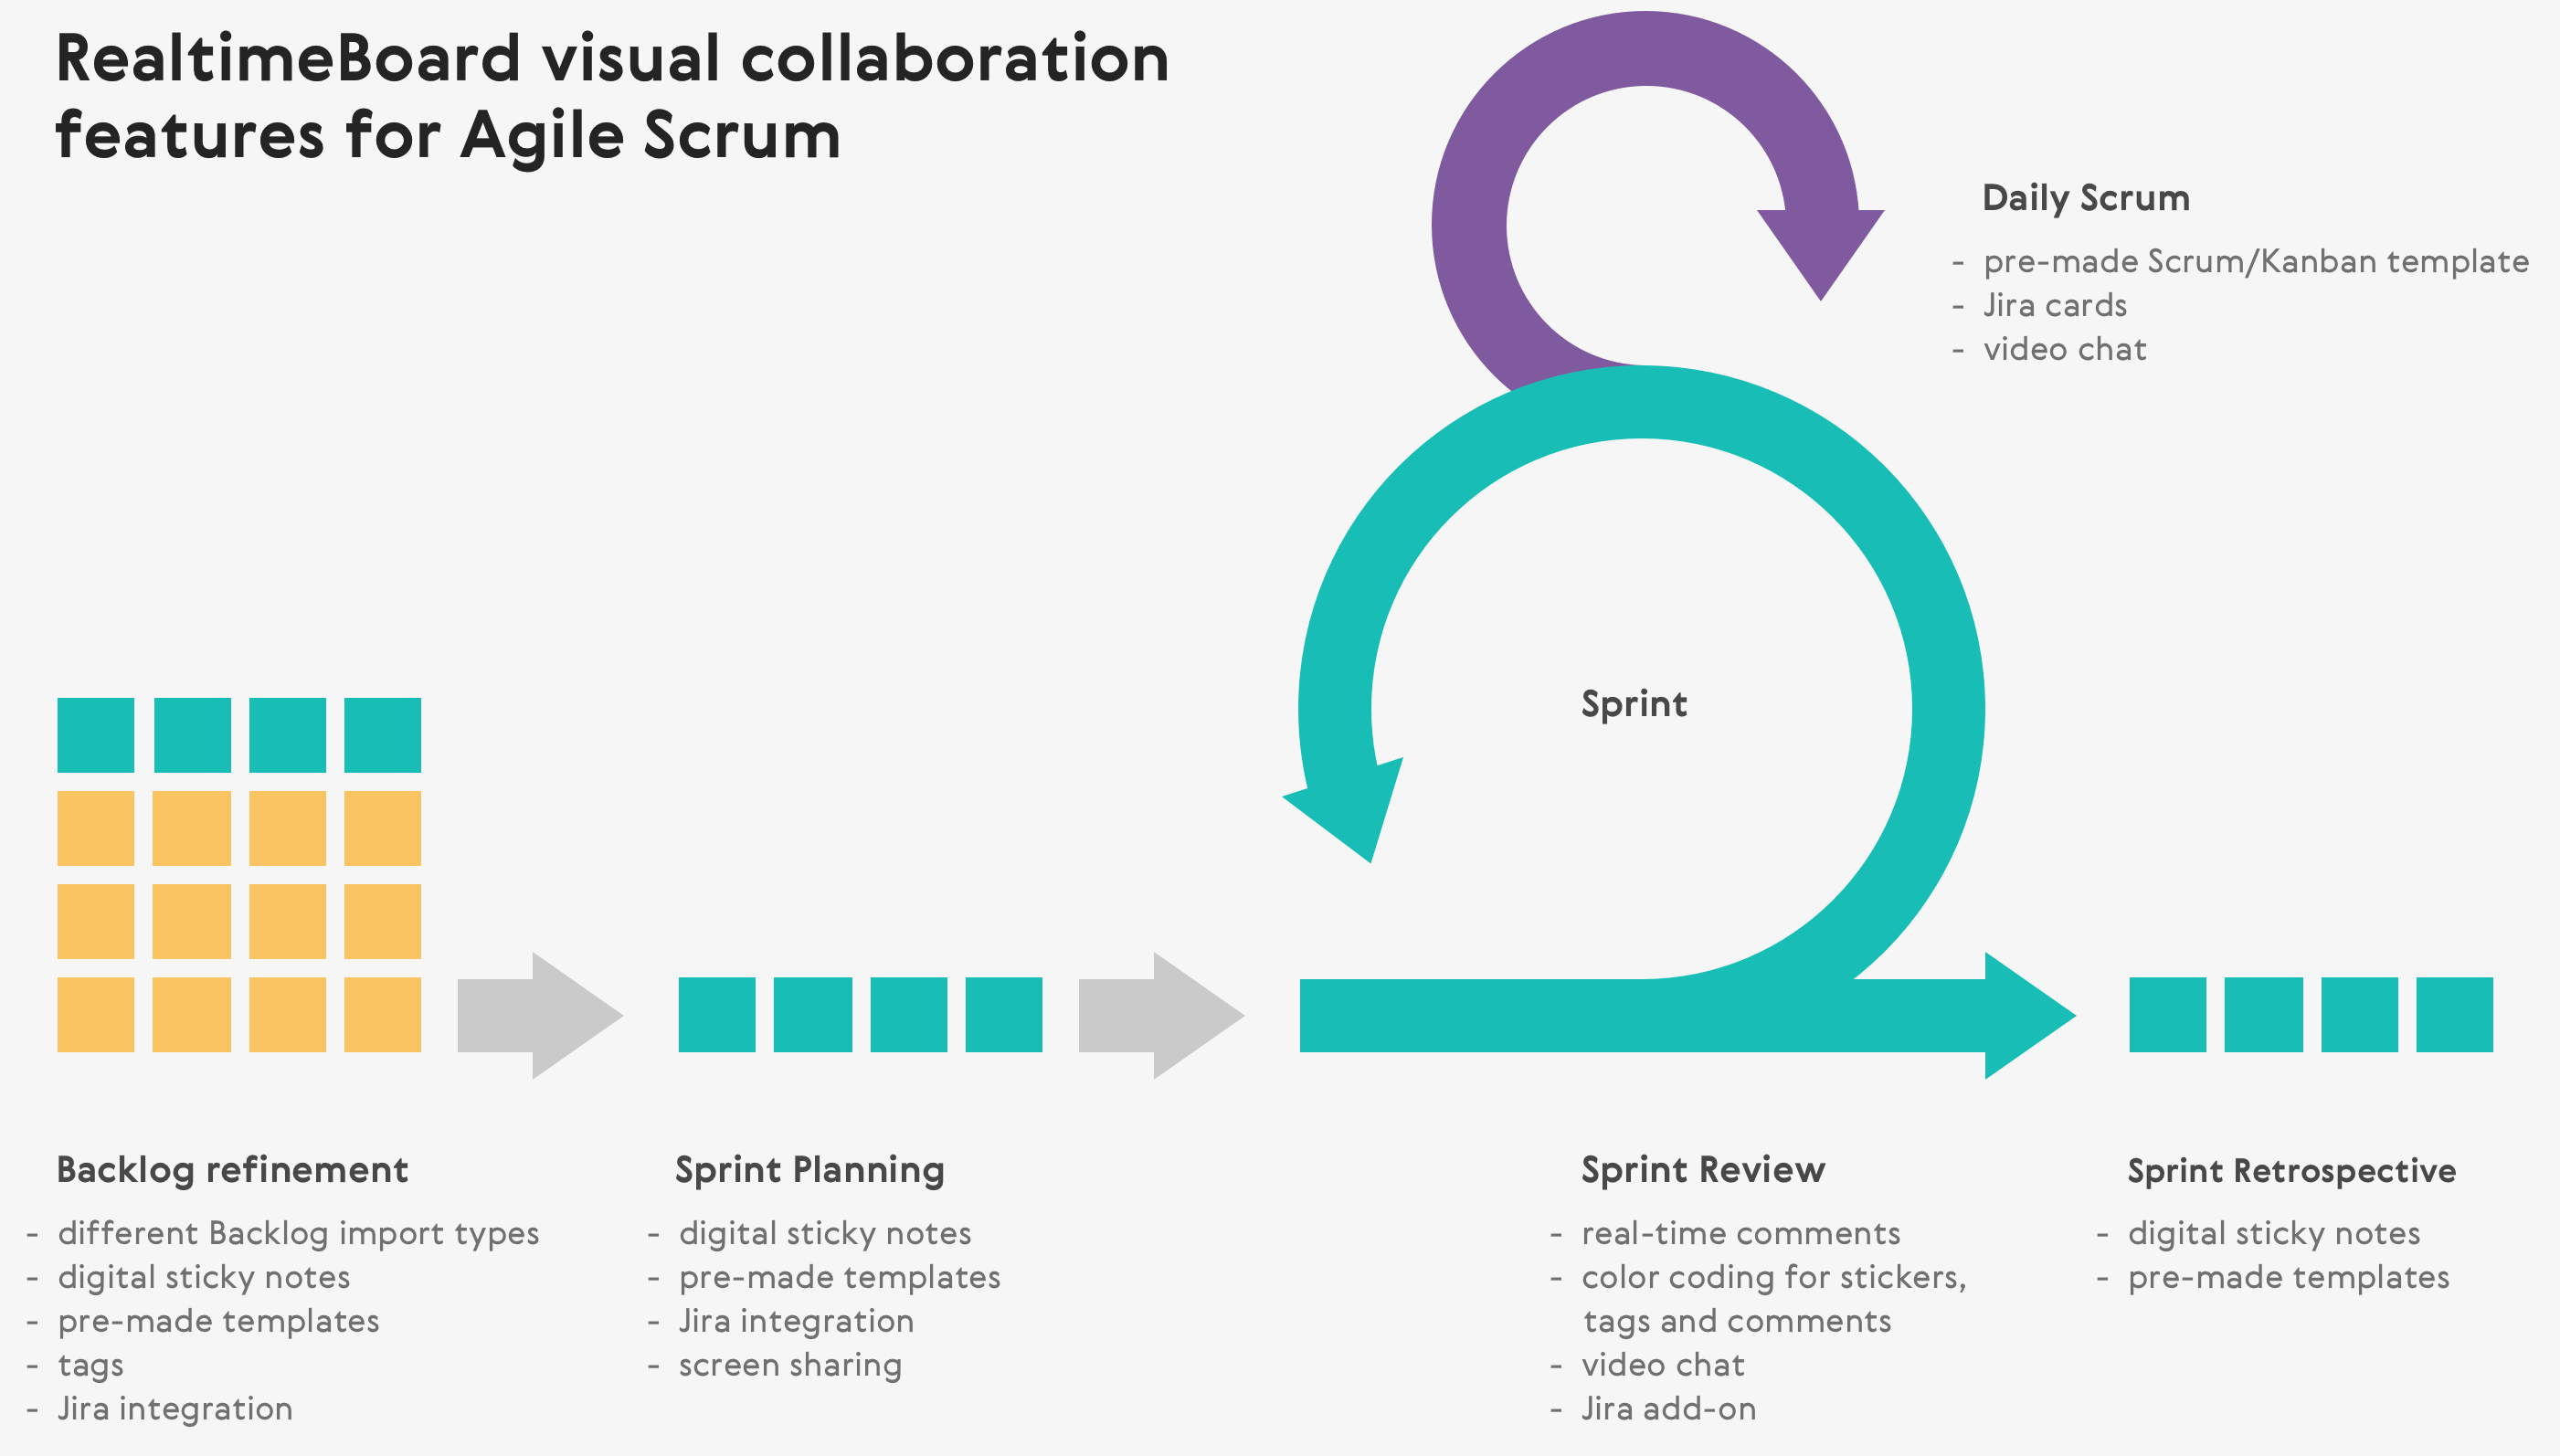
\includegraphics[scale=0.56]{img/rtb_scrum_agile_slide_2.png}
\newline
\begin{exampleblock}{Introduction}

The calculator exhibits the use of a certain ETERNITY:NUMBERS. The number which is included in the project is Gelfond's number. It is a transcendental number. It can be represented as $e^{\pi}$. The potential user base include the students, researchers and professionals from the physics and mathematics field. 

\end{exampleblock} 

%----------------------------------------------------------------------------------------

\begin{columns}[t,totalwidth=\twocolwid] % Split up the two columns wide column again

\begin{column}{\onecolwid} % The first column within column 2 (column 2.1)

%----------------------------------------------------------------------------------------
%	MATHEMATICAL SECTION
%----------------------------------------------------------------------------------------

\begin{exampleblock}{Critical Decisions}

1. Because the Gelfond's constant is not known to many researchers, it is difficult to identify the target market. The decision of keeping the constant in the product has several factors:

\begin{itemize}
\item It can be useful in the product considering the future possible use of the constant.
\item Since it has only couple applications, it is not likely to be used more frequently.

\vspace{1em}
2. The decision to choose the kind of user in-
\end{itemize}

\end{exampleblock}

%----------------------------------------------------------------------------------------

\end{column} % End of column 2.1
\begin{column}{\sepwid}\end{column} % Empty spacer column

\begin{column}{\onecolwid} % The second column within column 2 (column 2.2)

%----------------------------------------------------------------------------------------
%	RESULTS
%----------------------------------------------------------------------------------------

\begin{exampleblock}{Critical Decisions}

-terface is also critical. Though many researchers are familiar with command line interface. Some might prefer the GUI.

3. While constructing the domain model, the functions to include in the product was a difficult decision due to several reasons:
\begin{itemize}
    \item The researchers preferred more personalized product than a generic one
    \item The product design must cover the larger market in the physics.
\end{itemize}

\end{exampleblock}

%----------------------------------------------------------------------------------------

\end{column} % End of column 2.2

\end{columns} % End of the split of column 2

\end{column} % End of the second column

\begin{column}{\sepwid}\end{column} % Empty spacer column

\begin{column}{\onecolwid} % The third column

%----------------------------------------------------------------------------------------
%	CONCLUSION
%----------------------------------------------------------------------------------------

\begin{exampleblock}{Difficulties Faced}

\begin{itemize}
    \item Most of the research individuals do not use conventional social media platform, it was initially difficult to reach out to them.
    \item With limited information gathered about the ETERNITY:NUMBERS assigned from the target market, it was difficult to brainstorm about the persona and the target product.
    \item Prioritizing the user stories is one of the most difficult parts about the user stories.
    \item Coming up with the right reference point for the user stories in relevantly new product is a difficult task.
\end{itemize}

\end{exampleblock}

%----------------------------------------------------------------------------------------
%	ADDITIONAL INFORMATION
%----------------------------------------------------------------------------------------

\begin{exampleblock}{Lessons Learnt}

\begin{itemize}
    \item The market research is not fruitful unless you completely understand the problem domain.
    \item Brainstorming ideas with team members gives better vision to the product design.
    \item Each user story may not be related to the product interface. Some user stories define the internal functionality and may not show visible work for the customers.
    \item Estimating the user story points may not be accurate at the beginning. The accuracy comes with experience.
\end{itemize}

\end{exampleblock}

\centering
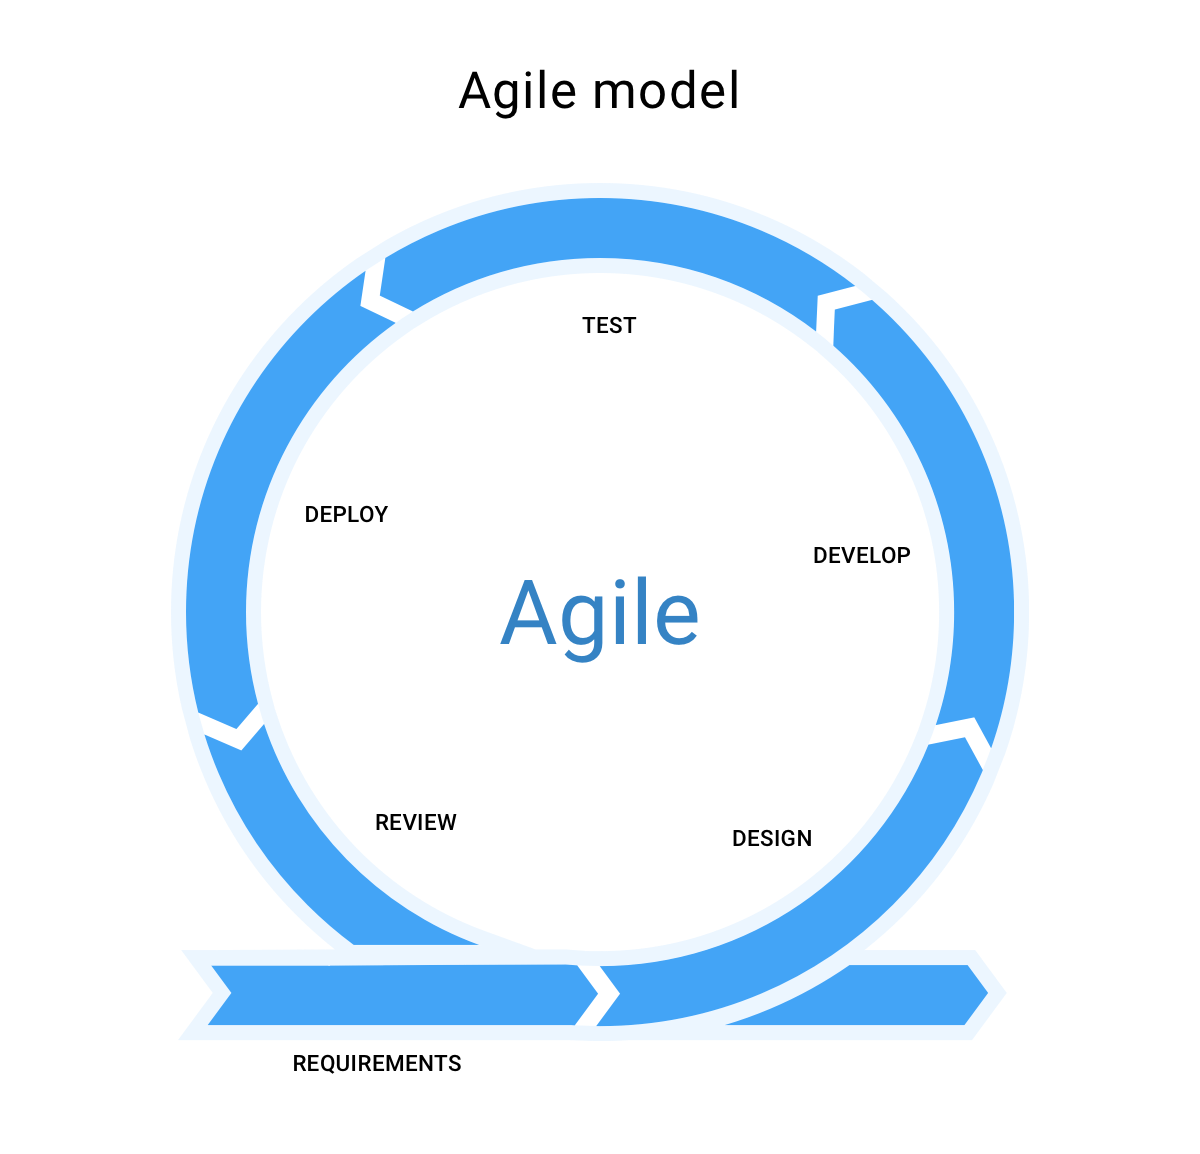
\includegraphics[scale=0.45]{img/agile-model.png}

%----------------------------------------------------------------------------------------

\end{column} % End of the third column

\begin{column}{\sepwid}\end{column} % Empty spacer column

\end{columns} % End of all the columns in the poster

\end{frame} % End of the enclosing frame
%\end{darkframes} % Uncomment for dark theme
\end{document}
